\documentclass[11pt, a4paper]{article}
\usepackage{fullpage}
\usepackage[USenglish]{babel}
\usepackage{graphicx} 
\usepackage[small,bf,hang]{caption2}
\usepackage{hyperref}
\hypersetup{
    colorlinks,
    citecolor=black,
    filecolor=black,
    linkcolor=black,
    urlcolor=black
}

\title{Master Thesis -  Security Aspects in Virtual Networks\\ \textbf{SITREP 13}}
\author{\textbf{Laurent De Wilde} \\ Master of Science in the Applied Computer Science \\ Vrije Universiteit Brussel}
\date{April 6, 2015}

\begin{document}
\maketitle

\section*{Work done}

This is an overview of the work performed in the past week:
\begin{itemize}
\item Hacked the virtual disk (vhdx) of a Hyper-V VM and placed a Trojan in the Startup folder, such that the Trojan connects to the attacker's computer and sets up a session with it, so that the attacker can easily obtain network information, execute programs and browse through files.
\item Placed a Trojan in the partition of the other OS of the dualboot system (from the first OS) and managed to start the Trojan when this other OS started up.
\end{itemize}
First of all, it appears that one can just mount a virtual hard disk with Windows Explorer, after which the disk partitions (including the ``System Reserved'' and the normal data partitions) appear in the Explorer window. Access is possible just by browsing the directories. We assume that a hacker has attacked the Hyper-V host and has root access to the system.
$\;$ \\ \\
\noindent\begin{minipage}{\textwidth}
    \centering
    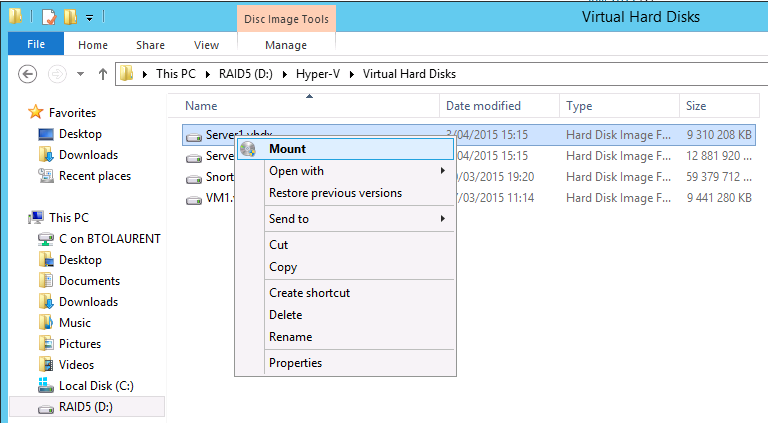
\includegraphics[width=\textwidth]{Mount_1.png}
 \captionof{figure}{Mounting the virtual hard disk in Windows Server 2012 R2 using Windows Explorer \ldots}
\end{minipage}
$\;$ \\ \\
\noindent\begin{minipage}{\textwidth}
    \centering
    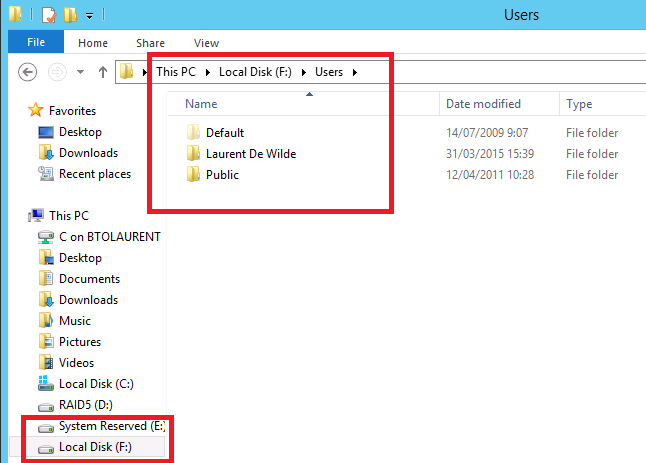
\includegraphics[width=\textwidth]{Mount_2.png}
 \captionof{figure}{\ldots after which the partitions become visible (browseable).}
\end{minipage}
$\;$ \\ \\
However, I discovered that once the VM has been started again, no access to the hard drive in Windows Explorer is possible anymore. So I created a Trojan Horse on my computer that I inserted into the hard drive of the compromised VM and that automatically connects to the computer of the attacker (my computer) once the VM has booted without the user being aware of it, after which I can browse files, see the network configuration etc etc \ldots .\\
This way, permanent access to the compromised VM is possible. \\
\noindent\begin{minipage}{\textwidth}
    \centering
    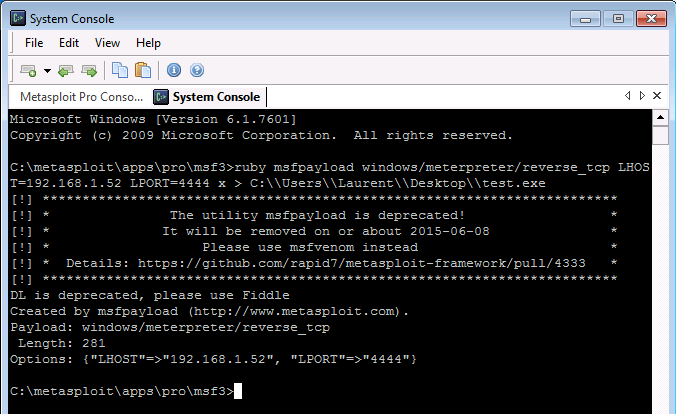
\includegraphics[width=\textwidth]{Payload_1.png}
 \captionof{figure}{Creation of the malicious Trojan.}
\end{minipage}
$\;$ \\ \\
\noindent\begin{minipage}{\textwidth}
    \centering
    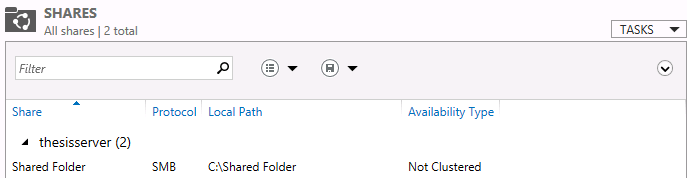
\includegraphics[width=\textwidth]{Shares_1.png}
 \captionof{figure}{Transferred the Trojan to the host by means of a shared folder.}
\end{minipage}
$\;$ \\ \\
\noindent\begin{minipage}{\textwidth}
    \centering
    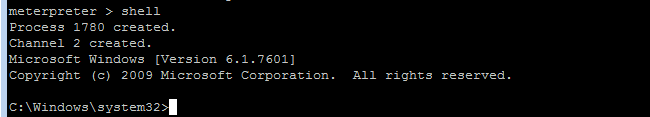
\includegraphics[width=\textwidth]{Shell_1.png}
 \captionof{figure}{Once the VM has started, it connects automatically to my computer and I can browse the files, even when the hard drive is in use and not mountable anymore in Windows Explorer.}
\end{minipage}
$\;$ \\ \\
\noindent\begin{minipage}{\textwidth}
    \centering
    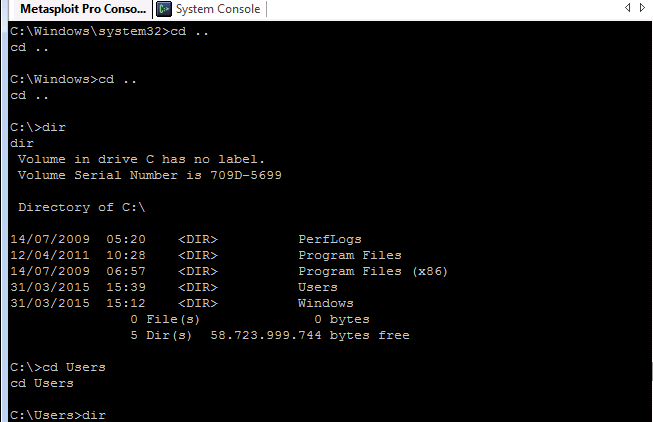
\includegraphics[width=\textwidth]{Shell_2.png}
 \captionof{figure}{An example of the directory listing of the compromised VM.}
\end{minipage}
$\;$ \\ \\
I showed that it is possible to break into a virtual hard disk and insert some virusses or trojans to infect a virtual machine trough the host.

\subsection*{Place a virus on the other dualboot system}

Using ``Dualboot2'', I managed to place a Trojan on ``Dualboot1''. When ``Dualboot1'' was started again, the Trojan was started as well and connected to the attacker's computer (my computer) as shown in the figures. The two dualboot systems are both Windows 7 Professional x64 editions. This is just an example, any other virus could be used. It is just to show that this is indeed possible.
$\;$ \\ \\
\noindent\begin{minipage}{\textwidth}
    \centering
    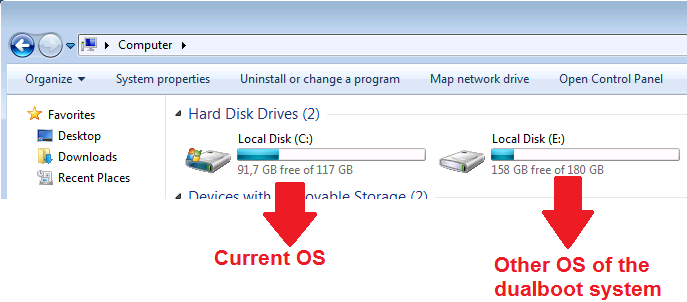
\includegraphics[width=\textwidth]{Hack_3.png}
 \captionof{figure}{The two disks of the two OS's visible in Windows Explorer.}
\end{minipage}
$\;$ \\ \\
The Trojan is placed in the Startup folder and will be executed when the OS boots. \\ \\
\noindent\begin{minipage}{\textwidth}
    \centering
    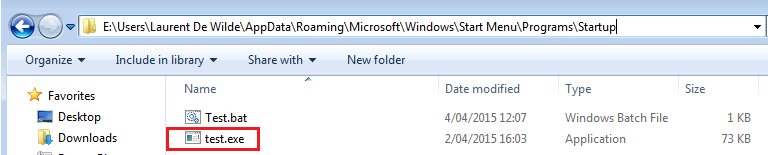
\includegraphics[width=\textwidth]{Hack_1.png}
 \captionof{figure}{The trojan is inserted in the other OS of the dualboot system.}
\end{minipage}
$\;$ \\ \\
With the Trojan connected to our computer, we can now browse files, etc etc \ldots . \\ \\
\noindent\begin{minipage}{\textwidth}
    \centering
    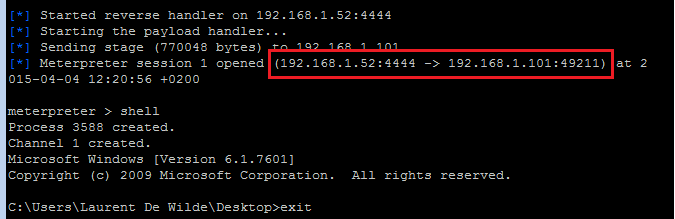
\includegraphics[width=\textwidth]{Hack_2.png}
 \captionof{figure}{The Trojan has connected to our computer.}
\end{minipage}


\section*{Planning}
\begin{itemize}
\item Investigate the problem with the broken Hard disk drive on the pizza server.
\item More in-depth break-out testing from a VM to the Hyper-V host.
\end{itemize}


\section*{Problems}



\section*{Issues}



\section*{Assistance}


\end{document}